%%%%%%%%%%%%%%%%%%%%%%%%%%%%%%%%%%%%%%%%%
% Wenneker Assignment
% LaTeX Template
% Version 2.0 (12/1/2019)
%
% This template originates from:
% http://www.LaTeXTemplates.com
%
% Authors:
% Vel (vel@LaTeXTemplates.com)
% Frits Wenneker
%
% License:
% CC BY-NC-SA 3.0 (http://creativecommons.org/licenses/by-nc-sa/3.0/)
% 
%%%%%%%%%%%%%%%%%%%%%%%%%%%%%%%%%%%%%%%%%

%----------------------------------------------------------------------------------------
%	PACKAGES AND OTHER DOCUMENT CONFIGURATIONS
%----------------------------------------------------------------------------------------

\documentclass[11pt]{scrartcl} % Font size

%%%%%%%%%%%%%%%%%%%%%%%%%%%%%%%%%%%%%%%%%
% Wenneker Assignment
% Structure Specification File
% Version 2.0 (12/1/2019)
%
% This template originates from:
% http://www.LaTeXTemplates.com
%
% Authors:
% Vel (vel@LaTeXTemplates.com)
% Frits Wenneker
%
% License:
% CC BY-NC-SA 3.0 (http://creativecommons.org/licenses/by-nc-sa/3.0/)
% 
%%%%%%%%%%%%%%%%%%%%%%%%%%%%%%%%%%%%%%%%%

%----------------------------------------------------------------------------------------
%	PACKAGES AND OTHER DOCUMENT CONFIGURATIONS
%----------------------------------------------------------------------------------------

\usepackage{amsmath, amsfonts, amsthm} % Math packages

\usepackage{listings} % Code listings, with syntax highlighting

\usepackage[english]{babel} % English language hyphenation

\usepackage{graphicx} % Required for inserting images
\usepackage{caption}
\graphicspath{{Figures/}{./}} % Specifies where to look for included images (trailing slash required)

\usepackage{booktabs} % Required for better horizontal rules in tables

\numberwithin{equation}{section} % Number equations within sections (i.e. 1.1, 1.2, 2.1, 2.2 instead of 1, 2, 3, 4)
\numberwithin{figure}{section} % Number figures within sections (i.e. 1.1, 1.2, 2.1, 2.2 instead of 1, 2, 3, 4)
\numberwithin{table}{section} % Number tables within sections (i.e. 1.1, 1.2, 2.1, 2.2 instead of 1, 2, 3, 4)

\setlength\parindent{0pt} % Removes all indentation from paragraphs

\usepackage{enumitem} % Required for list customisation
\setlist{noitemsep} % No spacing between list items

%----------------------------------------------------------------------------------------
%	DOCUMENT MARGINS
%----------------------------------------------------------------------------------------

\usepackage{geometry} % Required for adjusting page dimensions and margins

\geometry{
	paper=a4paper, % Paper size, change to letterpaper for US letter size
	top=2.5cm, % Top margin
	bottom=3cm, % Bottom margin
	left=3cm, % Left margin
	right=3cm, % Right margin
	headheight=0.75cm, % Header height
	footskip=1.5cm, % Space from the bottom margin to the baseline of the footer
	headsep=0.75cm, % Space from the top margin to the baseline of the header
	%showframe, % Uncomment to show how the type block is set on the page
}

%----------------------------------------------------------------------------------------
%	FONTS
%----------------------------------------------------------------------------------------

\usepackage[utf8]{inputenc} % Required for inputting international characters
\usepackage[T1]{fontenc} % Use 8-bit encoding

\usepackage{fourier} % Use the Adobe Utopia font for the document

%\usepackage[framed,numbered,autolinebreaks,useliterate]{mcode}

%----------------------------------------------------------------------------------------
%	SECTION TITLES
%----------------------------------------------------------------------------------------

\usepackage{sectsty} % Allows customising section commands

\sectionfont{\normalfont\bfseries} % \section{} styling
\subsectionfont{\normalfont\bfseries} % \subsection{} styling
\subsubsectionfont{\normalfont\itshape} % \subsubsection{} styling
\paragraphfont{\normalfont\scshape} % \paragraph{} styling

%----------------------------------------------------------------------------------------
%	HEADERS AND FOOTERS
%----------------------------------------------------------------------------------------

\usepackage{scrlayer-scrpage} % Required for customising headers and footers

\ohead*{} % Right header
\ihead*{} % Left header
\chead*{} % Centre header

\ofoot*{} % Right footer
\ifoot*{} % Left footer
\cfoot*{\pagemark} % Centre footer

% MY PACKAGES
%\usepackage[framed,numbered,autolinebreaks,useliterate]{mcode}
\usepackage{listings}
\usepackage{float}
\usepackage{amsmath}
\usepackage{tikz}
\usetikzlibrary{shapes,arrows,positioning}
\usepackage{hyperref} % Include the file specifying the document structure and custom commands

%----------------------------------------------------------------------------------------
%	TITLE SECTION
%----------------------------------------------------------------------------------------

\title{	
	\normalfont\normalsize
	\textsc{Universität Würzburg}\\ % Your university, school and/or department name(s)
	\vspace{25pt} % Whitespace
	\rule{\linewidth}{0.5pt}\\ % Thin top horizontal rule
	\vspace{20pt} % Whitespace
	{\huge Robotik II - Übung 01}\\ % The assignment title
	{\large Zustandsraummodell, Sprungantwort, Linearisierung}\\ % The assignment title
	\vspace{12pt} % Whitespace
	\rule{\linewidth}{2pt}\\ % Thick bottom horizontal rule
	\vspace{12pt} % Whitespace
}

\author{\LARGE Alexander Björk, Janis Kaltenthaler} % Your name

\date{\normalsize\today} % Today's date (\today) or a custom date

\begin{document}

\maketitle % Print the title

%----------------------------------------------------------------------------------------
%	FIGURE EXAMPLE
%----------------------------------------------------------------------------------------

\section*{Aufgabe 1-1. Fahrt mit der Eisenbahn (5 Punkte)}

\subsection*{a)}

Die Differenzialgeleichung, die sich nach dem zweiten Newtonschen Gesetz
\begin{equation*}
F=ma=m\dot{v}
\end{equation*}
ergibt, setzt sich aus der Beschleunigungs- bzw. Bremskraft der Lokomotive $u(t)$ und der durch den Rollwiderstand erzeugten Bremskraft $F_w(t)$ zusammen. Damit ergibt sich
\begin{equation*}
F=ma=m\dot{v}=u+F_w.
\end{equation*}
Setzt man für $F_w(t)$ den gegebenen Zusammenhang $c \cdot v(t)$ mit $c=1500 \dfrac{\text{kg}}{\text{s}}$ ein, erhält man die geforderte Differentialgelichung erster Ordnung
\begin{equation*}
m \cdot \dot{v}(t) = c \cdot v(t) + u(t).
\end{equation*}
Für die Überführung ins Zustandsraummodell wird $u(t)$ als Eingangsgröße und $v(t)$ sowohl als Zustands- als auch als Ausgangsgröße angenommen. Damit ergibt sich das Modell zu
\begin{equation*}
\dot{x}(t)=ax(t)+bu(t)
\end{equation*}
mit 
\begin{align*}
a &= -\dfrac{c}{m_{ges}} \quad \text{und} \\
b &= \dfrac{1}{m_{ges}}.
\end{align*}
$m_{ges}$ ist dabei die Gesamtmasse der Eisenbahn, die sich aus der Masse der Lokomotive und den 10 Wagen zusammensetzt.

\subsection*{b)}
Der Eigenwert der Systemmatrix $A=a$ des Zustandraummodells ergibt sich aufgrund der Eindimensionalität zu
\begin{align*}
\text{det}(A-\lambda I) &= 0 \\
a - \lambda &= 0 \\
\lambda &= -\dfrac{c}{m_{ges}}.
\end{align*}

\subsection*{c)}
Die Lösung der Bewegungsgleichung nach der beschriebenen Eingangsgröße wird wie in Folie 10 (Kapitel 02: Einführung dynamischer Systeme) nach
\begin{equation*}
y(t)=c^T\Phi(t)x_0+\int_{0}^{t}c^T\Phi(t-\tau)bu(\tau)d\tau + du(t)
\end{equation*}
berechnet. Durch die stückweise definierte Eingangsgröße muss hier jedoch auch stückweise vorgegangen werden. Die Lösung muss daher in drei Teilschritten berechnet und auch die Lösung muss anschließend stückweise angegeben werden.\\
Die Lösung vereinfacht sich durch die Eindimensionalität erheblich:
\begin{equation*}
x(t)=e^{a(t-t_0)}x_0+\int_{0}^{t}e^{a(t-(\tau)}bu(\tau)d\tau
\end{equation*}

Der \textbf{erste Abschnitt} ist für $t_0\leq t \leq t_1$ definiert. Somit gilt es
\begin{equation*}
x(t)=e^{a(t-t_0)}x_0+\int_{0}^{t}e^{a(t-(\tau)}bu(\tau)d\tau
\end{equation*}
zu lösen. Da man in diesem Intervall $u(\tau)$ als konstant annehmen kann, vereinfacht sich auch das Integral. Die Lösung ist 
\begin{equation*}
x(t)=e^{at}x_0 + \dfrac{b}{a} F_a (e^{at} - 1)
\end{equation*}
mit
\begin{equation*}
F_a = 80 \text{kN}.
\end{equation*}

Der \textbf{zweite Abschnitt} ist für $t_1 < t \leq t_2$ definiert. Somit gilt es
\begin{equation*}
x(t)=e^{a(t-t_1)}x(t_1)+\int_{t_1}^{t}e^{a(t-(\tau)}bu(\tau)d\tau
\end{equation*}
zu lösen. Da in diesem Intervall $u(\tau) = 0$ gilt, ist die Lösung 
\begin{equation*}
x(t)=e^{a(t-t_1)}x(t_1).
\end{equation*}

Der \textbf{dritte Abschnitt} ist für $t_2 < t \leq t_3$ definiert. Somit gilt es
\begin{equation*}
x(t)=e^{a(t-t_2)}x(t_2)+\int_{t_2}^{t}e^{a(t-(\tau)}bu(\tau)d\tau
\end{equation*}
zu lösen. In diesem Intervall kann $u(\tau)$ erneut als konstant angenommen werden. Die Lösung ist
\begin{equation*}
x(t)=e^{a(t-t_2)}x(t_2) + \dfrac{b}{a} F_b (e^{a(t-t_2)} - 1)
\end{equation*}
mit
\begin{equation*}
F_b = -90 \text{kN}.
\end{equation*}

Die endgültige Lösung ist damit
\begin{equation*}
x(t) = \left\{
        \begin{array}{lll}
            e^{at}x_0 + \dfrac{b}{a} F_a (e^{at} - 1) & \quad t_0\leq t \leq t_1 \\
            e^{a(t-t_1)}x(t_1) & \quad \text{sonst} \\
            e^{a(t-t_2)}x(t_2) + \dfrac{b}{a} F_b (e^{a(t-t_2)} - 1) & \quad t_2 < t \leq t_3.
        \end{array}
    \right.
\end{equation*}

\subsection*{d)}
\begin{figure}[H]
	\centering
	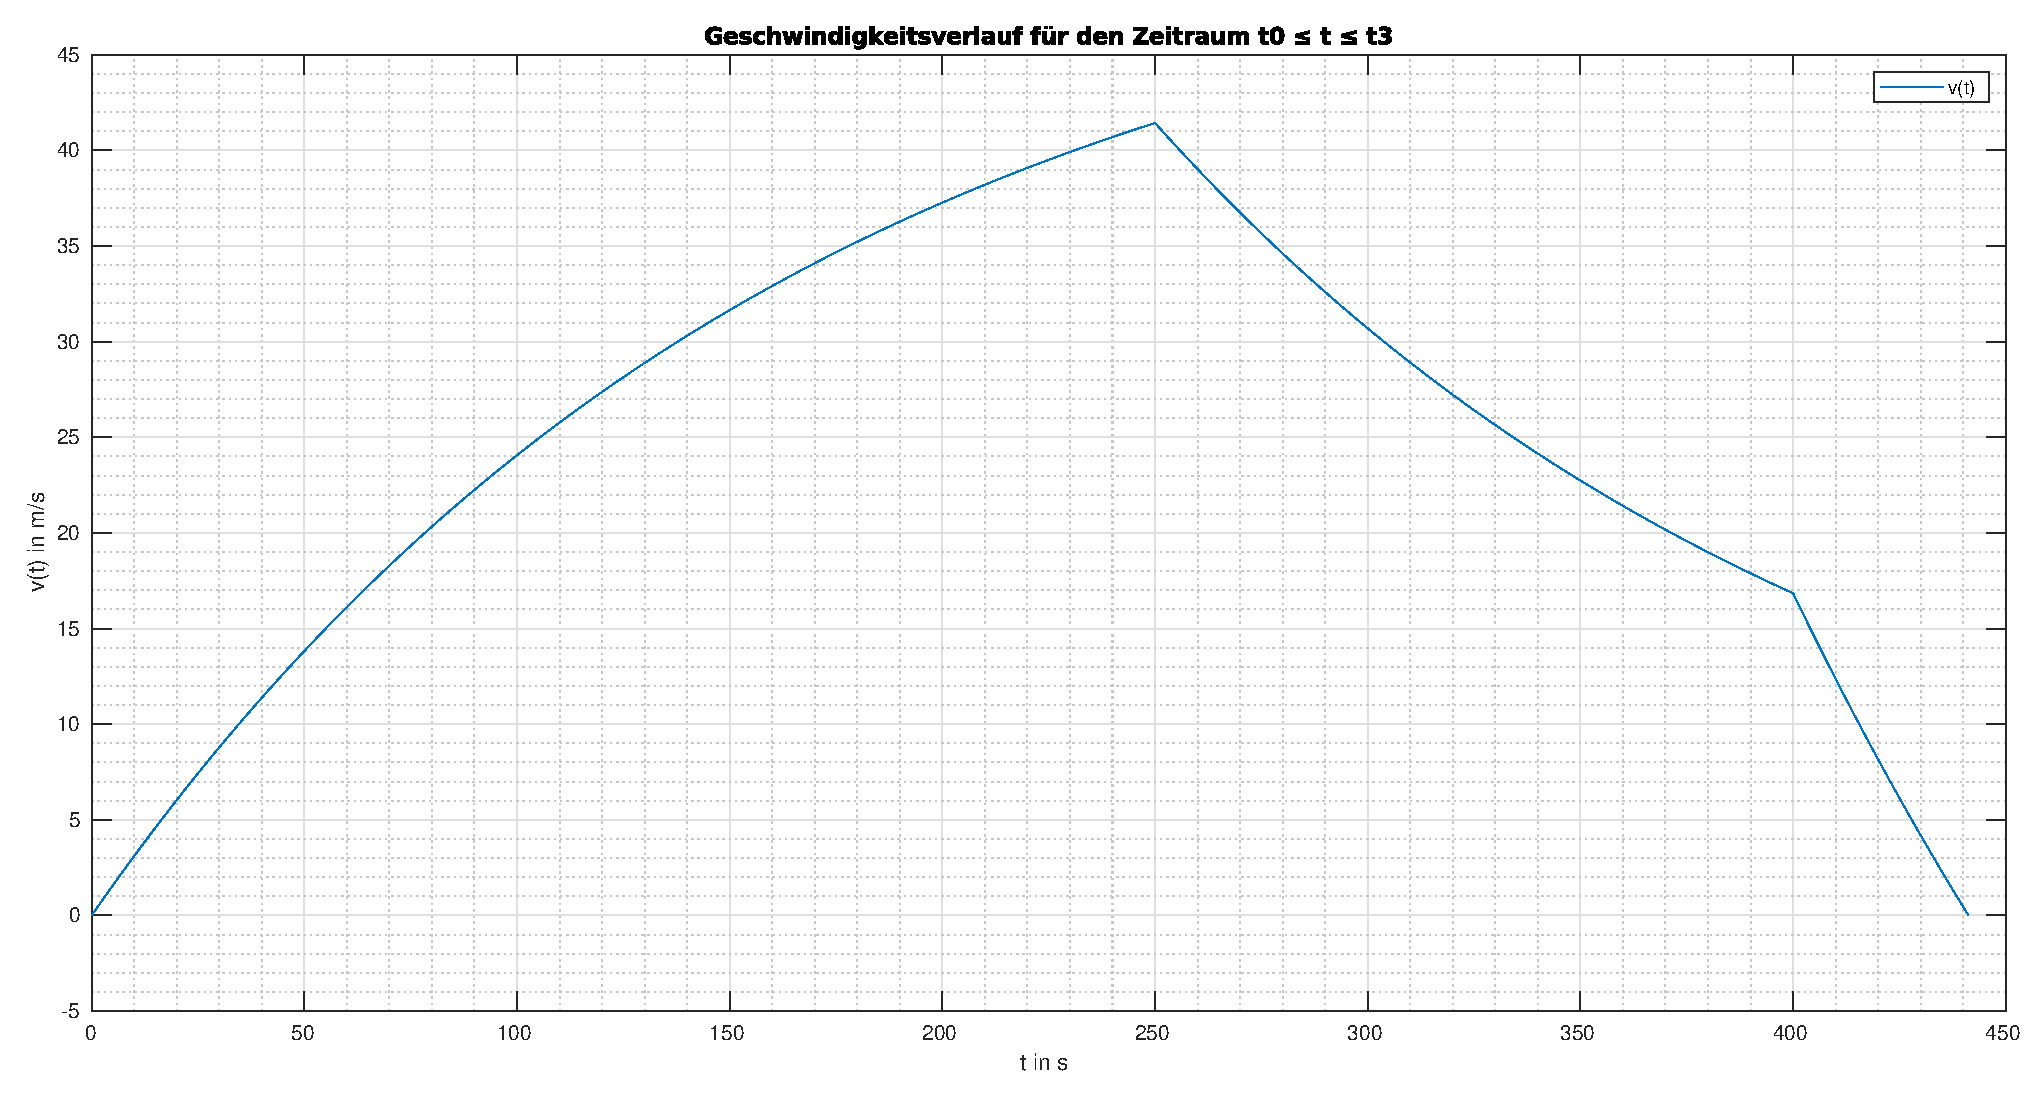
\includegraphics[width=\textwidth]{speed.eps}
	\captionsetup{labelformat=empty}
	\caption{Abb. 1.1: Geschwindigkeitsverlauf für $t_0 \leq t \leq t_3$}
\end{figure}

\begin{figure}[H]
	\centering
	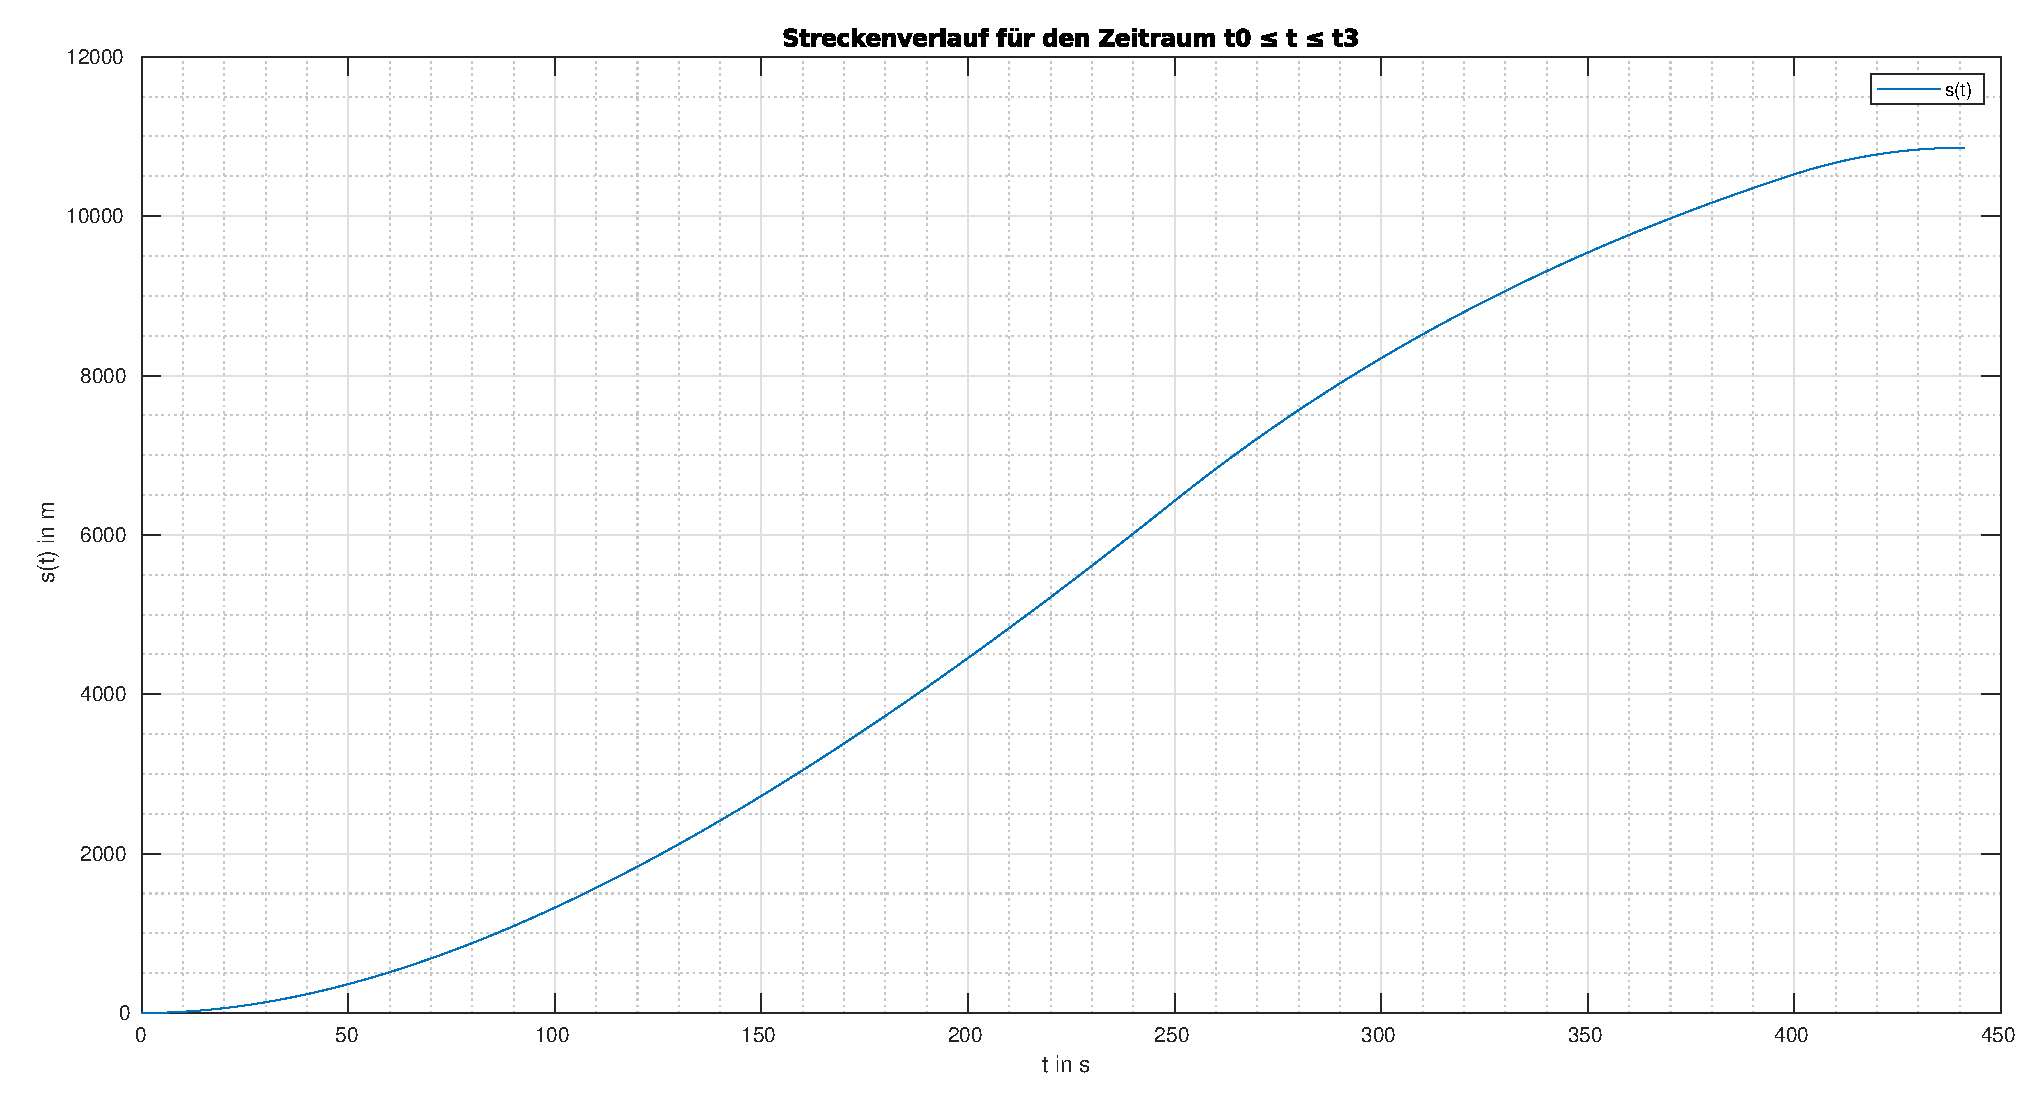
\includegraphics[width=\textwidth]{dist.eps}
	\captionsetup{labelformat=empty}
	\caption{Abb. 1.2: Streckenverlauf für $t_0 \leq t \leq t_3$}
\end{figure}


%------------------------------------------------

\section*{Aufgabe 1-2. Simulation und Linearisierung eines Pendels am Wagen (5 Punkte)}

\subsection*{b)}
Der Wagen wird aus dem anfänglichen Ruhepunkt $x = 0$ ausgeschwungen und pendelt danach um einen von Null verschiedenen Punkt (in der Simulation ungefähr ${x = 0.015}$). Dabei ist die Amplitude während einer Schwingungsdauer nahezu synchron mit der Amplitude der Pendelgeschwindigkeit. Nach ungefähr 30 Sekunden ist die Position des Wagens nahezu konstant und die Wagengeschwindigkeit somit nahezu Null. Das Pendel jedoch schwingt noch, nun relativ gleichmäßig.

\subsection*{c)}
Die linearisierten Zustandsgleichungen für $\ddot{x}$ und $\ddot{\theta}$ sehen wie folgt aus:
\begin{align*}
\ddot{x} &= T \left( \dfrac{F}{m} - \dfrac{{m_p}^2l^2}{Jm}g\theta + \dfrac{m_pl}{Jm}f_p\theta - \dfrac{f_c}{m} \dot{x} \right)\\[15pt]
\ddot{\theta} &= T \left( \dfrac{m_pl}{J} g \theta - \dfrac{m_pl}{Jm}F + \dfrac{m_pl}{Jm} f_c \dot{x} - \dfrac{f_p}{J} \dot{\theta} \right)
\end{align*}
mit
\begin{equation*}
T = \dfrac{1}{1 - \dfrac{{m_p}^2l^2}{Jm}}.
\end{equation*}

Dadurch ergibt sich das linearisierte Zustandsraummodell zu

\begin{align*}
\dot{\vec{x}} &= 
\begin{bmatrix}
0 & 1 & 0 & 0\\
0 & -T \cdot \dfrac{f_c}{m} & -T \cdot \dfrac{{m_p}^2l^2}{Jm}g & T \cdot \dfrac{m_p l}{Jm}f_p\\
0 & 0 & 0 & 1\\
0 & T \cdot \dfrac{m_p l}{Jm}f_c & T \cdot \dfrac{m_p l}{J}g & -T \cdot \dfrac{f_p}{J}
\end{bmatrix} 
\vec{x}
+
\begin{bmatrix}
0\\
T\dfrac{1}{m}\\
0\\
-T\dfrac{m_pl}{Jm}
\end{bmatrix}
u
\\[25pt]
y &= 
\begin{bmatrix}
1 & 0 & 0 & 0\\
0 & 0 & 1 & 0
\end{bmatrix}
\vec{x}.
\end{align*}

\subsection*{e)}

\begin{figure}[H]
	\centering
	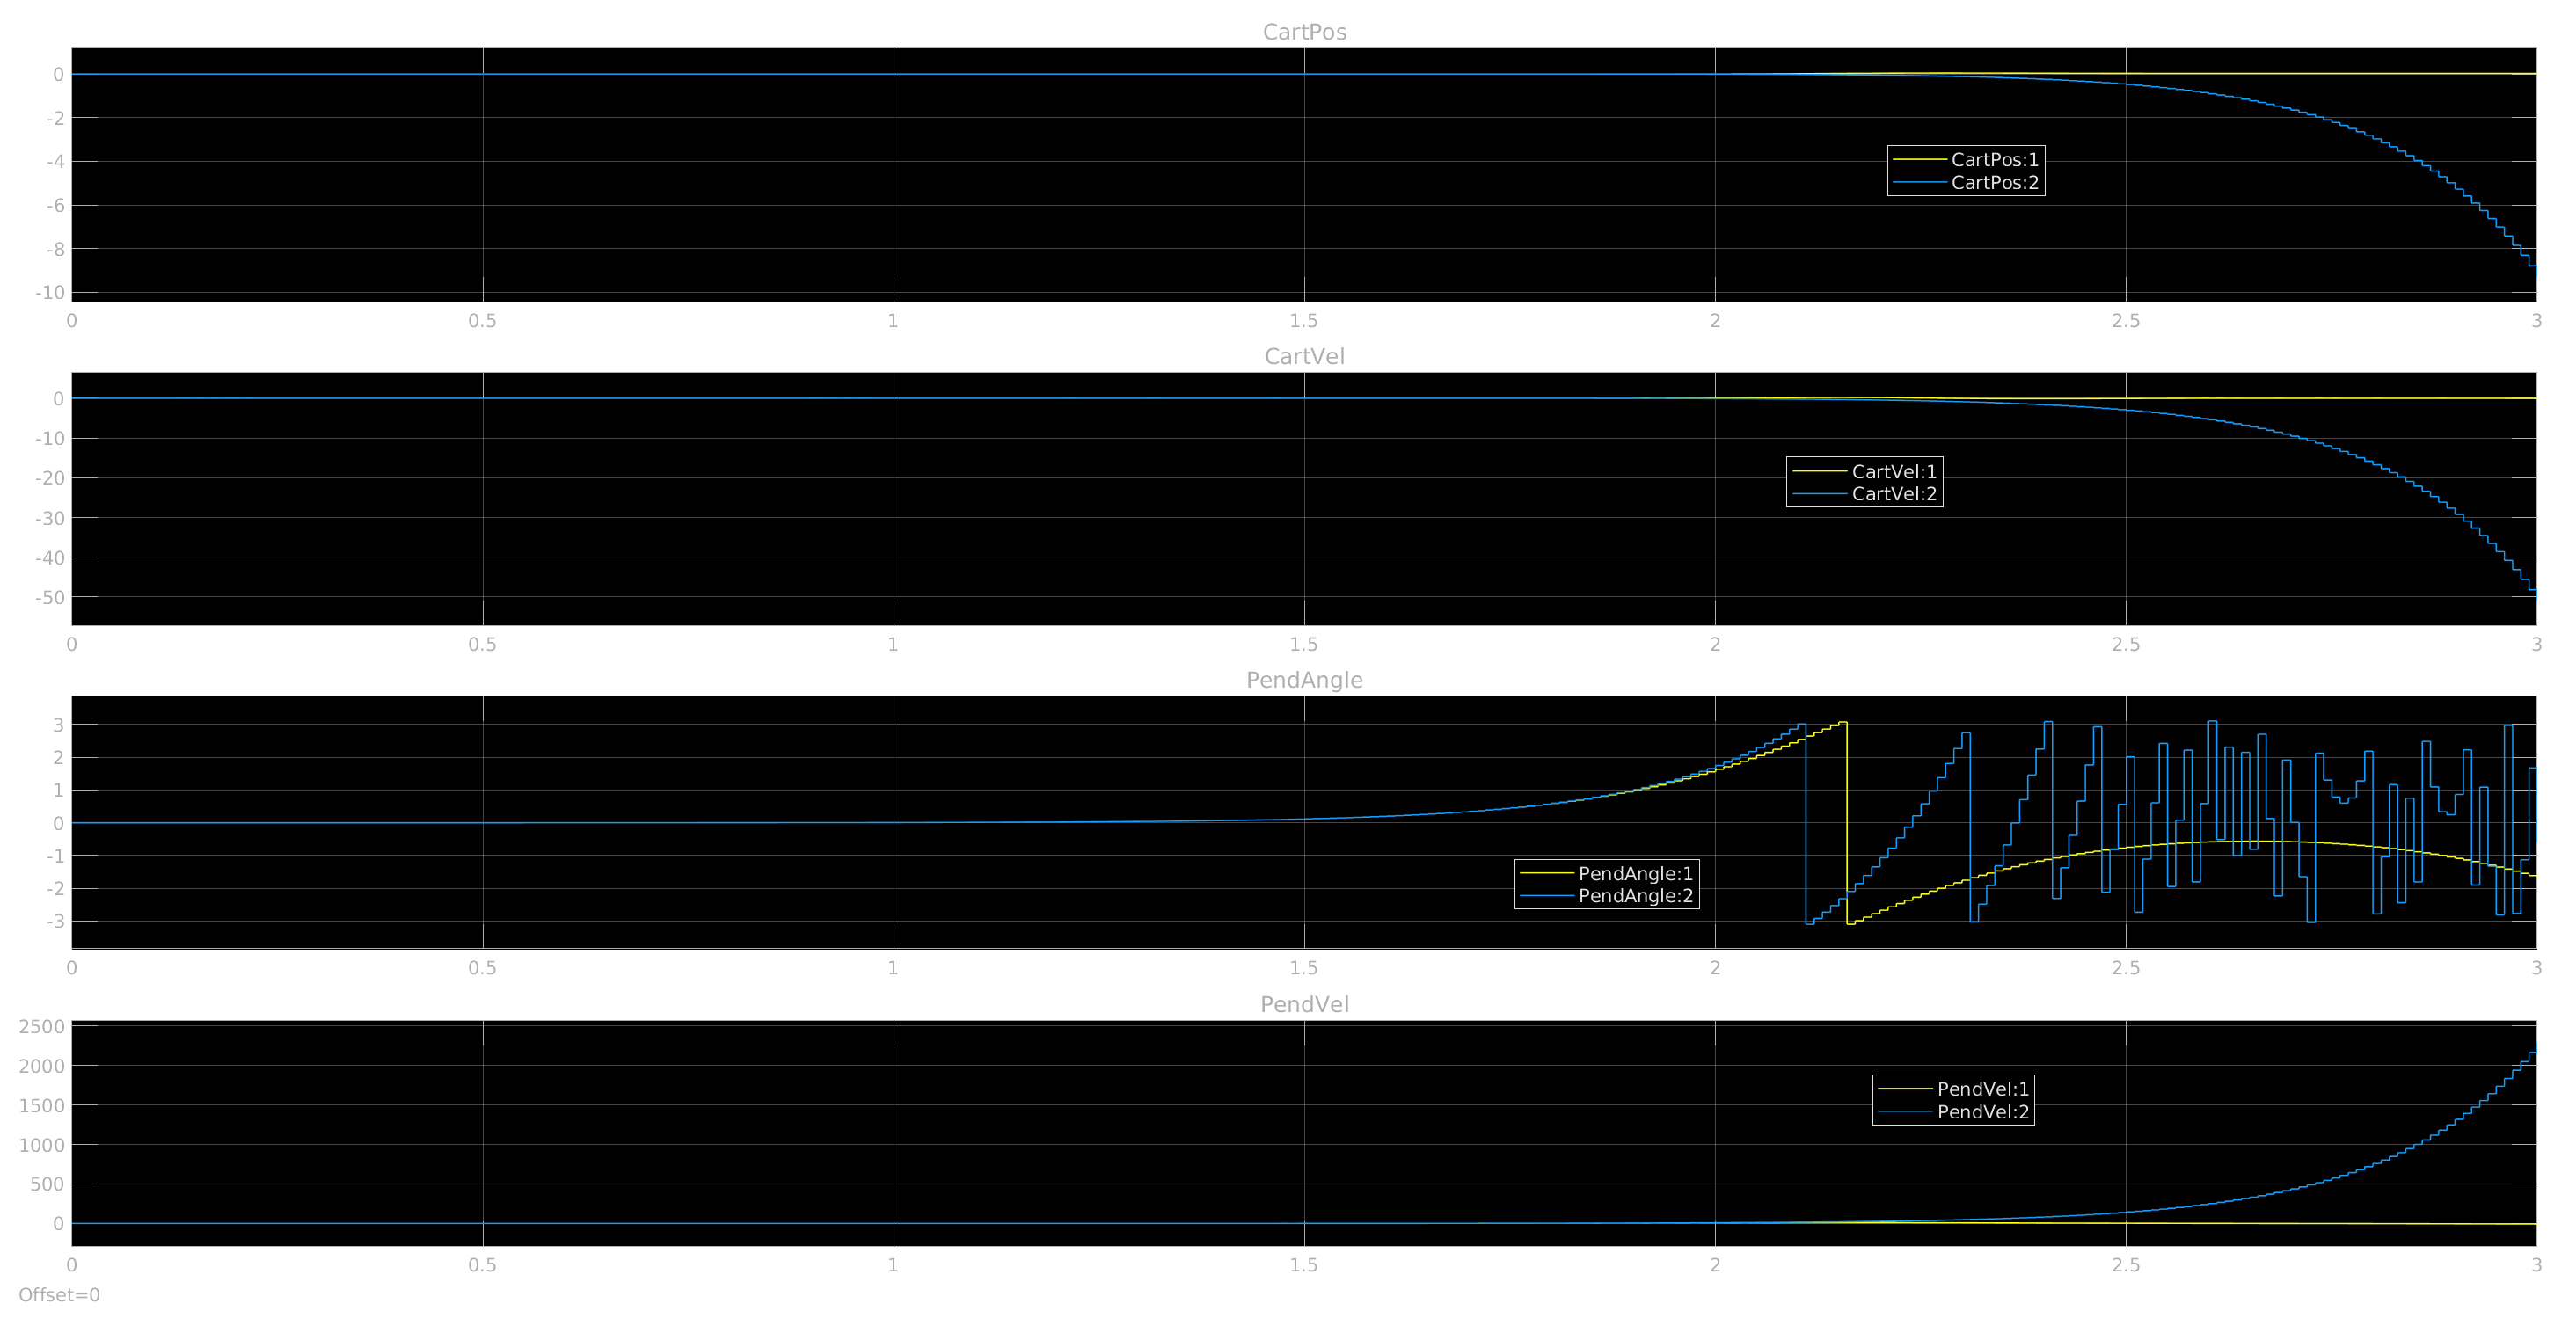
\includegraphics[width=\textwidth]{pendel.eps}
	\captionsetup{labelformat=empty}
	\caption{Abb. 2.1: Scope des nichtlinearen (gelb) und linearen (blau) Pendels}
\end{figure}

Im kleinen $\theta$-Bereich, also der Bereich in dem die Linearisierung gültig ist, stimmen die Ausgaben überein. Die Linearisierung ist also tatsächlich gültig. Ist die Auslenkung des Pendels jedoch zu groß, ist die Linearisierung nicht mehr gültig, was in den Ausgaben auch eindeutig zu sehen ist.



\end{document}
